\documentclass[11pt]{article}

\usepackage[margin=0.65in]{geometry}
\usepackage{tikz}
\usepackage{amsmath}

\usetikzlibrary{
    arrows.meta,
    positioning,
    calc,
    fit,
    backgrounds
}

\pagestyle{empty}

\begin{document}

\begin{figure}[t]
\centering

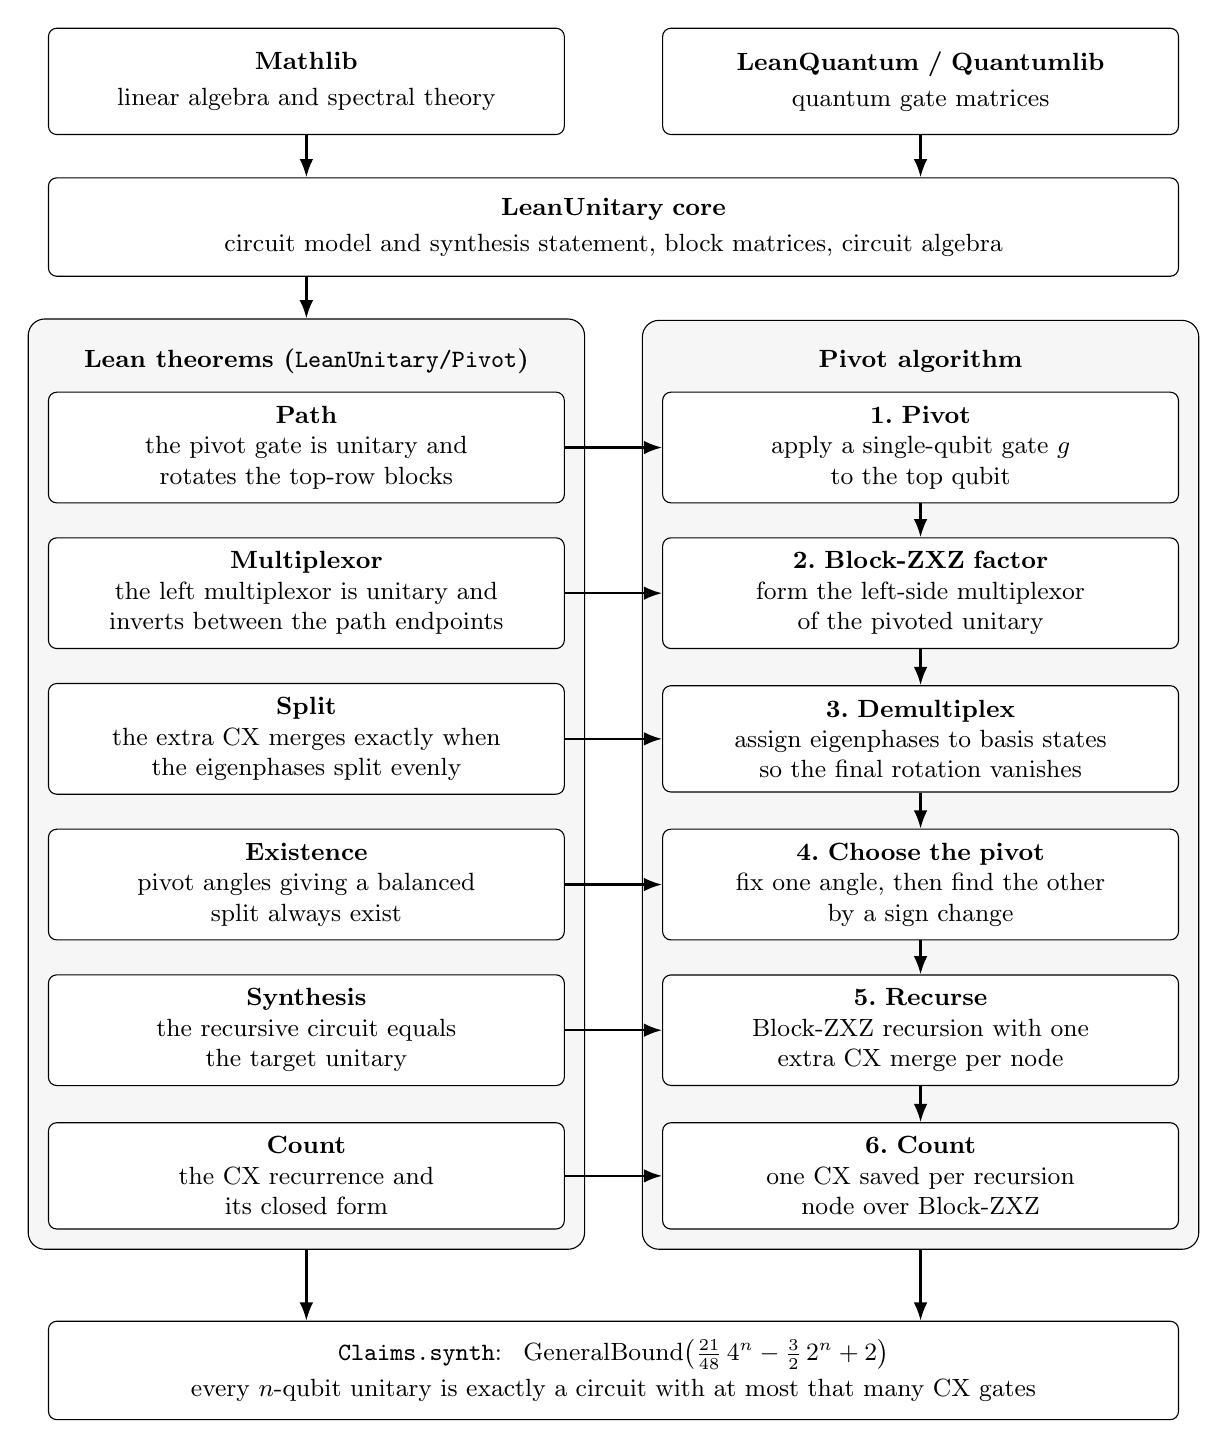
\begin{tikzpicture}[
    >=Latex,
    font=\small,
    box/.style={
        draw,
        rounded corners=3pt,
        align=center,
        inner sep=5pt,
        fill=white
    },
    col/.style={box, text width=6.2cm, minimum height=1.35cm},
    wide/.style={box, text width=14.0cm, minimum height=1.25cm},
    head/.style={font=\small\bfseries, text width=6.2cm, align=center},
    arrow/.style={->, thick}
]

\def\xl{-3.9}
\def\xr{3.9}
\def\dy{1.85}

% ============================================================
% FORMAL CONTEXT
% ============================================================

\node[col] (mathlib) at (\xl,0) {
    \textbf{Mathlib}\\[2pt]
    linear algebra and spectral theory
};

\node[col] (quantum) at (\xr,0) {
    \textbf{LeanQuantum / Quantumlib}\\[2pt]
    quantum gate matrices
};

\node[wide] (core) at (0,-\dy) {
    \textbf{LeanUnitary core}\\[2pt]
    circuit model and synthesis statement, block matrices, circuit algebra
};

\draw[arrow] (mathlib.south) -- (mathlib.south |- core.north);
\draw[arrow] (quantum.south) -- (quantum.south |- core.north);

% ============================================================
% THEOREMS (left) VERIFY THE ALGORITHM (right)
% ============================================================

\node[head] (hl) at (\xl,-3.55) {Lean theorems (\texttt{LeanUnitary/Pivot})};
\node[head] (hr) at (\xr,-3.55) {Pivot algorithm};

\newcommand{\row}[3]{%
    \node[col] (t#1) at (\xl,{-2.8-#1*\dy}) {#2};
    \node[col] (a#1) at (\xr,{-2.8-#1*\dy}) {#3};
    \draw[arrow] (t#1.east) -- (a#1.west);
}

\row{1}{\textbf{Path}\\the pivot gate is unitary and\\rotates the top-row blocks}
    {\textbf{1.\ Pivot}\\apply a single-qubit gate $g$\\to the top qubit}
\row{2}{\textbf{Multiplexor}\\the left multiplexor is unitary and\\inverts between the path endpoints}
    {\textbf{2.\ Block-ZXZ factor}\\form the left-side multiplexor\\of the pivoted unitary}
\row{3}{\textbf{Split}\\the extra CX merges exactly when\\the eigenphases split evenly}
    {\textbf{3.\ Demultiplex}\\assign eigenphases to basis states\\so the final rotation vanishes}
\row{4}{\textbf{Existence}\\pivot angles giving a balanced\\split always exist}
    {\textbf{4.\ Choose the pivot}\\fix one angle, then find the other\\by a sign change}
\row{5}{\textbf{Synthesis}\\the recursive circuit equals\\the target unitary}
    {\textbf{5.\ Recurse}\\Block-ZXZ recursion with one\\extra CX merge per node}
\row{6}{\textbf{Count}\\the CX recurrence and\\its closed form}
    {\textbf{6.\ Count}\\one CX saved per recursion\\node over Block-ZXZ}

\foreach \i [evaluate=\i as \j using int(\i+1)] in {1,...,5} {
    \draw[arrow] (a\i.south) -- (a\j.north);
}

\begin{scope}[on background layer]
\node[draw, rounded corners=6pt, fill=gray!7, inner sep=0.25cm,
    fit=(hl) (t1) (t6)] (lean) {};
\node[draw, rounded corners=6pt, fill=gray!7, inner sep=0.25cm,
    fit=(hr) (a1) (a6)] (alg) {};
\end{scope}

\draw[arrow] (core.south -| lean.north) -- (lean.north);

% ============================================================
% CLAIM
% ============================================================

\node[wide, below=0.9cm of $(lean.south)!0.5!(alg.south)$] (claim) {
    \mbox{\textbf{\texttt{Claims.synth}}: \
    $\mathrm{GeneralBound}\big(\tfrac{21}{48}\,4^n-\tfrac32\,2^n+2\big)$}\\[2pt]
    every $n$-qubit unitary is exactly a circuit with at most that many CX gates
};

\draw[arrow] (lean.south) -- (lean.south |- claim.north);
\draw[arrow] (alg.south) -- (alg.south |- claim.north);

\end{tikzpicture}

\caption{
Lean formalization of our proposed pivot decomposition. Each theorem module on the left
verifies the step of the pivot algorithm on its right, on top of Mathlib's linear
algebra and the circuit model of LeanUnitary. Together they give the CX bound
stated in \texttt{Claims.synth}.
}

\label{fig:lean-unitary}

\end{figure}

\end{document}
